\documentclass[12pt]{article}

% --- Packages ---
\usepackage[margin=1in]{geometry}
\usepackage{amsmath,amssymb}
\usepackage{booktabs}
\usepackage{natbib}
\usepackage{graphicx}
\usepackage{hyperref}
\usepackage{setspace}
\usepackage{caption}
\usepackage{subcaption}
\usepackage{threeparttable}
\usepackage{dcolumn}
\usepackage{float}
\usepackage{enumitem}
\usepackage[T1]{fontenc}
\usepackage{appendix}

\doublespacing

\hypersetup{
  colorlinks=true,
  linkcolor=blue,
  citecolor=blue,
  urlcolor=blue
}

\newcolumntype{d}[1]{D{.}{.}{#1}}

\title{\textbf{Missing Mass and Minimum Wages:\\
Distributional Effects of Three Minimum Wage Increases in Peru}}

\author{
  Carlos C\'esar Ch\'avez Padilla\thanks{Center for the Economics of Human Development, University of Chicago. Email: \texttt{cchavezpadilla@uchicago.edu}. I thank James J.\ Heckman for guidance and support. All errors are my own.}
}

\date{March 2026\\[6pt] \small\textit{Preliminary draft --- do not circulate}}

\begin{document}

\maketitle

\begin{abstract}
\noindent
I study the distributional effects of three minimum wage (MW) increases in Peru---from S/750 to S/1,025 between 2016 and 2022---using a pre-post distributional estimator adapted from Cengiz et al.\ (2019) for a national MW setting without control jurisdictions. Using ENAHO household survey data covering 9,000--11,700 formal dependent workers per year, I document clear missing mass below the old MW floor and excess mass above the new floor in all three events. Bunching ratios range from 0.70 to 0.83: for every 100 jobs that disappear from below the new minimum, 70--83 reappear above it. Placebo tests at artificial thresholds produce ratios 7 times smaller, confirming the signal is MW-specific. Results are replicated on EPE Lima quarterly data with tighter 6-month event windows. Employment effects cannot be identified: event-study pre-trends fail, the Kaitz instrumental variable is weak ($F < 3$), and panel attrition exceeds 76\%. Hours show no adjustment ($\leq \pm 1.1$h/week). Wage compression of 3--7 percentage points is present but 41--92\% is mechanical composition. The dominant effect of Peru's MW increases within the studied Kaitz range (0.52--0.57) is redistribution of the formal wage distribution, not measurable job destruction.

\medskip
\noindent\textbf{JEL Codes}: J31, J38, O17

\noindent\textbf{Keywords}: minimum wage, bunching estimator, wage distribution, Peru, informality
\end{abstract}

\newpage
\tableofcontents
\newpage

%=============================================================
\section{Introduction}\label{sec:intro}
%=============================================================

Peru raised its minimum wage (\textit{Remuneraci\'on M\'inima Vital}, RMV) three times between 2016 and 2022, from S/750 to S/1,025---a cumulative 37\% nominal increase. Throughout this period, formal employment remained stable and the formality rate recovered from its COVID-19 dip. What happened to the wage distribution? Did workers near the minimum wage floor receive raises, or did they lose their jobs?

This paper uses a pre-post distributional estimator inspired by the framework of \citet{cengiz2019}, adapted for Peru's national MW setting, to answer these questions. The estimator compares the formal wage distribution before and after each MW increase, measuring ``missing mass'' below the old threshold and ``excess mass'' at the new one. The ratio of excess to missing mass---the bunching ratio---indicates what fraction of displaced jobs reappear above the new floor.

The key challenge is that Peru has a single national MW with no sub-national variation in the policy. \citet{cengiz2019} construct their counterfactual by comparing U.S.\ states with MW changes to states without---a difference-in-differences design. This is not feasible in Peru. Instead, I follow the methodological precedent of \citet{harasztosi2016}, who analyze Hungary's national MW using the pre-reform wage distribution as the counterfactual, with a background correction from the upper tail of the distribution.

I analyze three MW events: Event A (S/750$\to$S/850, May 2016), Event B (S/850$\to$S/930, April 2018), and Event C (S/930$\to$S/1,025, May 2022). Using ENAHO household survey data from 2015--2023, covering approximately 10,000 formal dependent workers per year, I find bunching ratios of 0.696, 0.829, and 0.830 for the three events respectively. Bootstrap 95\% confidence intervals are [0.567, 0.896], [0.716, 1.016], and [0.716, 0.960]. Events A and C reject $R = 1$ (full redistribution with zero job loss); Event B does not---the data are consistent with both complete redistribution and displacement of up to 28\% of affected workers.

Placebo tests at artificial thresholds (S/1,100$\to$S/1,200 and S/1,400$\to$S/1,500) produce ratios of 0.114 and 0.013, with missing mass 7 times smaller than at the true MW---confirming the bunching signal is MW-specific. Results are stable across aligned bin widths (S/10--S/25; see Section~\ref{sec:results}) and across populations. An independent dataset---EPE Lima quarterly data with 6-month event windows---produces consistent ratios (0.73--1.03 vs.\ ENAHO's 0.70--0.83).

I systematically test three identification strategies for employment effects: department-level event-study DiD, Kaitz instrumental variables at department and province levels, and within-year province IV. All fail. Event-study pre-trends are violated for Events B ($p = 0.007$) and C ($p = 0.017$); Event A has no testable pre-period. The Kaitz IV produces $F$-statistics below 3 in all specifications, far below the Stock-Yogo threshold. The ENAHO panel has 76\% attrition with differential selection by treatment group. These failures are not data-quality issues but a structural feature of single-national-MW settings: Kaitz variation across departments reflects poverty gradients with independent secular and seasonal dynamics.

The paper contributes to the MW literature in three ways. First, it provides the first distributional analysis of Peru's MW using three identifiable events, contributing to the growing evidence base from developing countries \citep[see][]{harasztosi2016, saltiel2018, gindling2021, engbom2022}. The broader debate on whether MW increases reduce or merely redistribute employment has not reached consensus \citep{card1994, neumark2022, manning2021, dube2019}; \citet{belman2014} survey over 200 studies and find wide variation driven by methodology and context. This paper contributes a systematic identification of what can and cannot be learned in a national-MW setting. Second, it documents the systematic failure of regression-based identification in a national-MW setting, offering a methodological cautionary note for researchers working in similar institutional contexts. Third, by decomposing apparent wage compression into mechanical (composition) and genuine components, it clarifies that 41--92\% of measured compression reflects MW-induced worker sorting, not spillover wage effects.

%=============================================================
\section{Institutional Context}\label{sec:context}
%=============================================================

\subsection{Peru's Minimum Wage System}

The \textit{Remuneraci\'on M\'inima Vital} (RMV) is set by executive decree and applies to all registered formal dependent workers (\textit{empleados} and \textit{obreros}). It is not indexed to inflation or productivity and changes only when the government issues a new decree. Enforcement is conducted by SUNAFIL (\textit{Superintendencia Nacional de Fiscalizaci\'on Laboral}), with inspections concentrated in Lima and large firms.

Peru's labor market is characterized by high informality: approximately 72--75\% of employed workers are informal by INEI's comprehensive definition \citep{chacaltana2001, jaramillo2006, diaz2014}. The MW directly affects roughly 10--15\% of the workforce classified as formal dependent workers under INEI's formality variable (\texttt{ocupinf == 2}), which requires social security registration or a written employment contract.

\subsection{The Three MW Events}

Table~\ref{tab:events} summarizes the three MW changes analyzed in this paper. Each event is separated by at least two years, allowing clean pre-post comparisons using annual ENAHO surveys.

\begin{table}[H]
\centering
\caption{Minimum Wage Events Analyzed}
\label{tab:events}
\begin{threeparttable}
\begin{tabular}{lccccl}
\toprule
Event & Pre-MW & Post-MW & Change & Effective & Analysis years \\
\midrule
A & S/750 & S/850 & +13.3\% & May 2016 & Pre: 2015, Post: 2017 \\
B & S/850 & S/930 & +9.4\% & April 2018 & Pre: 2017, Post: 2019 \\
C & S/930 & S/1,025 & +10.2\% & May 2022 & Pre: 2021, Post: 2023 \\
\bottomrule
\end{tabular}
\begin{tablenotes}
\small
\item \textit{Note}: No 2020 survey due to COVID-19. Event C's pre-period (2021) reflects post-pandemic labor market conditions.
\end{tablenotes}
\end{threeparttable}
\end{table}

\subsection{Department-Level Kaitz Variation}

The Kaitz index (MW divided by the weighted-median formal wage by department) ranges from 0.39 to 1.09 across departments and years. Ica (department 11) has the highest Kaitz (0.94 in 2015), driven by formal agricultural workers on agro-export farms earning near-minimum monthly wages despite full-time hours (median 48 hours/week). Huancavelica (department 09) has a low Kaitz ($\approx 0.50$) because approximately 85\% of its formal workers are public-sector employees earning above the MW.

This variation primarily reflects differences in economic structure---the shares of agriculture and public-sector employment---rather than differential MW exposure. It does not generate sufficient first-stage power for IV identification ($F < 3$ in all events; see Appendix~\ref{app:iv}), and employment pre-trends fail for Events B and C (Appendix~\ref{app:eventstudy}). The Kaitz index is used in this paper as a descriptive measure of MW bindingness, not as an instrument.

%=============================================================
\section{Data}\label{sec:data}
%=============================================================

\subsection{ENAHO Module 500}

The primary data source is the \textit{Encuesta Nacional de Hogares} (ENAHO) Module 500 (\textit{Empleo e Ingresos}), conducted annually by INEI. I use cross-sectional data from eight years: 2015--2019, 2021--2023 (no 2020 survey due to COVID-19).

The analysis sample consists of formal dependent workers with monthly wages between S/1 and S/6,000 and positive survey weights. The filter chain is: employed (\texttt{ocu500 == 1}), dependent worker (\texttt{p507} $\in \{3, 4, 6\}$: \textit{empleado}, \textit{obrero}, \textit{trabajador del hogar}), formal (\texttt{ocupinf == 2}), wage $\in (0, 6000)$, weight $> 0$. The wage variable is \texttt{p524a1} (monthly cash income from primary occupation). The weight variable is \texttt{fac500a}. Department is identified from the first two digits of \texttt{ubigeo}.

\subsection{Summary Statistics}

Table~\ref{tab:summary} presents summary statistics for the analysis sample across all eight years.

\begin{table}[H]
\centering
\caption{Summary Statistics --- Formal Dependent Workers, ENAHO 2015--2023}
\label{tab:summary}
\begin{threeparttable}
\small
\begin{tabular}{lrrrrrrrr}
\toprule
 & 2015 & 2016 & 2017 & 2018 & 2019 & 2021 & 2022 & 2023 \\
\midrule
MW (S/.) & 750 & 850 & 850 & 930 & 930 & 930 & 1,025 & 1,025 \\
$N$ & 10,059 & 11,488 & 10,895 & 11,723 & 10,922 & 8,946 & 9,554 & 9,838 \\
Median wage & 1,400 & 1,500 & 1,500 & 1,673 & 1,700 & 1,800 & 1,800 & 1,863 \\
\% at MW & 4.6 & 4.8 & 6.0 & 4.8 & 6.5 & 7.8 & 5.7 & 8.2 \\
\% below MW & 10.9 & 14.0 & 10.4 & 14.6 & 12.5 & 11.5 & 16.9 & 12.6 \\
Median Kaitz & 0.536 & 0.567 & 0.567 & 0.556 & 0.547 & 0.517 & 0.569 & 0.550 \\
Mean hrs/wk & 46.4 & 46.2 & 46.4 & 46.3 & 46.2 & 46.8 & 46.6 & 46.5 \\
Formality (\%) & 26.7 & 27.9 & 27.4 & 27.6 & 27.3 & 23.2 & 24.3 & 26.1 \\
\bottomrule
\end{tabular}
\begin{tablenotes}
\small
\item \textit{Note}: $N$ = unweighted formal dependent workers with monthly wage S/1--6,000 and positive survey weight. \% at MW = share earning MW$\pm$25 (one bin). \% below MW = share earning below MW. Median Kaitz = MW / median wage, national. Formality rate = formal dependent / all employed. COVID-19 year 2021 shows depressed formality.
\end{tablenotes}
\end{threeparttable}
\end{table}

Median wages rise from S/1,400 (2015) to S/1,863 (2023), a 33\% nominal increase that roughly tracks the 37\% MW increase. The Kaitz index ranges from 0.517 to 0.569 with no clear trend; it does not monotonically increase over time. The share below MW rises sharply in pre-event years (14.0\% in 2016, 14.6\% in 2018, 16.9\% in 2022) and then falls as wages adjust to the new floor. Weekly hours are stable at 46--47 hours throughout the period.

%=============================================================
\section{Empirical Strategy}\label{sec:strategy}
%=============================================================

\subsection{Pre-Post Distributional Estimator}\label{sec:bunching}

I use a pre-post distributional estimator inspired by the framework of \citet{cengiz2019}, adapted for a national MW setting without control jurisdictions. \citet{cengiz2019} construct the counterfactual using U.S.\ states that did not raise their MW. Peru has a single national MW; I use the pre-period wage distribution with a background correction from the upper tail ($>2 \times \text{MW}_\text{new}$) instead. The closer methodological precedent is \citet{harasztosi2016}, who study Hungary's national MW.

The wage distribution is discretized into S/25 bins over the range S/0--S/6,000, weighted by survey expansion factors (\texttt{fac500a}). For each bin $b$, I compute the share of the workforce in the pre-period ($s_b^\text{pre}$) and post-period ($s_b^\text{post}$), and compute the raw delta: $\Delta_b = s_b^\text{post} - s_b^\text{pre}$.

The counterfactual correction uses an inverse-absolute-weighted average of $\Delta_b$ in the ``clean zone'' (bins with centers above $2 \times \text{MW}_\text{new}$), where the MW is unlikely to affect the distribution:
\[
\bar{\Delta}_\text{clean} = \frac{\sum_{b \in \mathcal{C}} w_b \cdot \Delta_b}{\sum_{b \in \mathcal{C}} w_b}, \quad w_b = \frac{1}{|\Delta_b| + \epsilon}
\]
where $\epsilon = 10^{-8}$. The adjusted delta is $\Delta_b^\text{adj} = \Delta_b - \bar{\Delta}_\text{clean}$.

Bins with $|\Delta_b| \approx 0$ receive higher weight because they represent wage regions where the pre-to-post change is minimal, providing the cleanest estimate of the background trend. The weighting prevents a small number of bins with anomalously large movements---which may reflect sector shocks rather than MW effects---from dominating the correction. Table~\ref{tab:sensitivity} shows results are robust to uniform weighting and alternative clean zone thresholds.

\textbf{Missing mass} (negative-only bins in the affected zone):
\begin{equation}
B^\text{miss} = \sum_{\substack{b \in [0.85 \times \text{MW}_\text{old},\; \text{MW}_\text{new}) \\ \Delta_b^\text{adj} < 0}} \left| \Delta_b^\text{adj} \right|
\end{equation}

\textbf{Excess mass} (positive-only bins in the excess zone):
\begin{equation}
B^\text{exc} = \sum_{\substack{b \in [\text{MW}_\text{new},\; \text{MW}_\text{new} + 250) \\ \Delta_b^\text{adj} > 0}} \Delta_b^\text{adj}
\end{equation}

The \textbf{bunching ratio} is $R = B^\text{exc} / B^\text{miss}$. A ratio of 1 indicates perfect redistribution: all displaced workers reappear above the new MW. A ratio below 1 indicates that some fraction of the missing mass does not reappear, consistent with job loss, informalization, or transitions beyond the S/250 excess window.

This estimator does not require between-unit parallel trends and is valid for all three events. It does assume that the upper tail of the distribution ($> 2 \times \text{MW}_\text{new}$) provides a valid counterfactual for background wage growth in the MW-relevant range. This assumption could be violated if high-wage and low-wage formal employment have different cyclical dynamics---for example, if recessions disproportionately contract low-wage formal employment. The placebo tests in Section~\ref{sec:results} provide a within-sample check: if the upper-tail correction were systematically biased, false-positive bunching signals would appear at artificial thresholds.

\subsection{Bootstrap Inference}

Standard errors are computed by block-bootstrapping individuals within each pre/post cross-section (1,000 replications). For each bootstrap draw, I resample with replacement and recompute the full bunching ratio. The 95\% confidence interval is the 2.5th and 97.5th percentiles of the bootstrap distribution.

\subsection{Hours DiD}

The intensive-margin hours response is measured by a 2$\times$2 DiD of weighted mean weekly hours (\texttt{p513t}). The treatment group is workers in the affected wage zone $[0.85 \times \text{MW}_\text{old}, \text{MW}_\text{new})$ in the pre-period and $[\text{MW}_\text{new}, 1.3 \times \text{MW}_\text{new}]$ in the post-period (tracking where displaced workers land). The control group is workers in $[1.5 \times \text{MW}_\text{new}, 3.0 \times \text{MW}_\text{new}]$ in both periods.

\subsection{Failed Identification Strategies (Appendices B--C)}

I attempted three regression-based identification strategies for employment effects, all of which fail. The event-study DiD uses department-level Kaitz variation; pre-trends are violated for Events B ($p = 0.007$) and C ($p = 0.017$). The Kaitz IV produces $F$-statistics of 1.5, 2.6, and 0.1---all far below the Stock-Yogo threshold. See Appendices~\ref{app:eventstudy} and~\ref{app:iv} for details.

%=============================================================
\section{Bunching Results}\label{sec:results}
%=============================================================

\subsection{Main Estimates}

Table~\ref{tab:bunching} presents the bunching estimates for all three events and three populations.

\begin{table}[H]
\centering
\caption{Pre-Post Bunching Estimates --- ENAHO Cross-Section}
\label{tab:bunching}
\begin{threeparttable}
\begin{tabular}{llccc}
\toprule
Event & Group & Missing (pp) & Excess (pp) & Ratio \\
\midrule
\textbf{A} (750$\to$850) & Formal dep & 6.78 & 4.72 & 0.696 \\
 & Informal dep & 4.45 & 5.42 & 1.218 \\
 & All workers & 5.41 & 4.72 & 0.872 \\[4pt]
\textbf{B} (850$\to$930) & Formal dep & 8.03 & 6.66 & 0.829 \\
 & Informal dep & 5.28 & 5.21 & 0.987 \\
 & All workers & 6.44 & 5.81 & 0.901 \\[4pt]
\textbf{C} (930$\to$1,025) & Formal dep & 13.02 & 10.80 & 0.830 \\
 & Informal dep & 5.50 & 4.46 & 0.811 \\
 & All workers & 8.29 & 6.84 & 0.824 \\
\bottomrule
\end{tabular}
\begin{tablenotes}
\small
\item \textit{Note}: Missing (pp) = share lost from $[0.85 \times \text{MW}_\text{old}, \text{MW}_\text{new})$ using negative-only bins. Excess (pp) = share gained at $[\text{MW}_\text{new}, \text{MW}_\text{new} + 250)$ using positive-only bins. Background correction: inverse-abs-weighted mean from clean zone ($> 2 \times \text{MW}_\text{new}$). Bins: S/25, range S/0--6,000.
\end{tablenotes}
\end{threeparttable}
\end{table}

\begin{figure}[H]
\centering
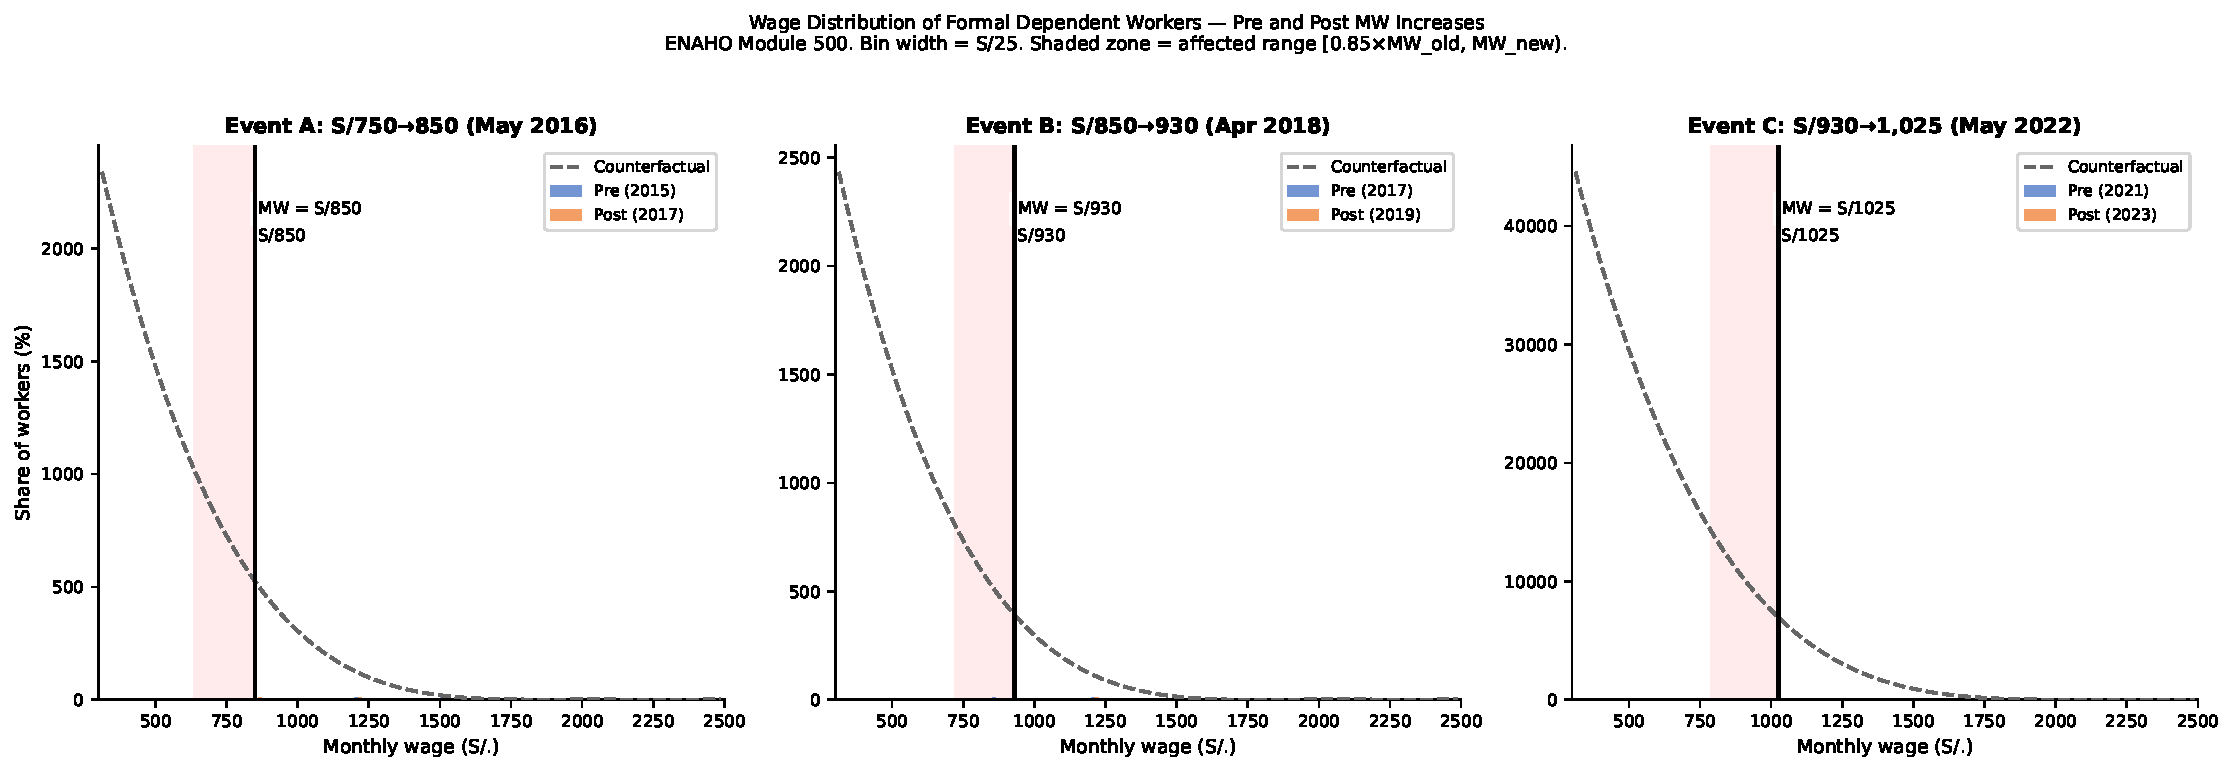
\includegraphics[width=\textwidth]{../exports/figures/fig2_bunching_distributions.pdf}
\caption{Wage Distributions Before and After MW Increases}
\label{fig:bunching}
{\small \textit{Note}: Three panels show the formal dependent wage distribution (S/25 bins, weighted by \texttt{fac500a}) before (blue) and after (orange) each MW increase. Vertical lines mark the old (dashed gray) and new (solid red) MW. Shaded region = affected zone $[0.85 \times \text{MW}_\text{old}, \text{MW}_\text{new})$.}
\end{figure}

Formal dependent workers show ratios consistently below 1 across all three events (0.696--0.830), indicating that more workers leave the affected zone than reappear at the new MW. Missing mass increases from 6.78pp (Event A) to 13.02pp (Event C), reflecting the growing MW bite as the RMV rises relative to the wage distribution.

Table~\ref{tab:effective_n} reports the unweighted observation counts in the affected and excess zones, confirming that the bunching signal is not driven by sparse cells. The affected zone contains 829--1,163 observations pre-policy; the excess zone contains 1,566--1,657 observations post-policy.

\begin{table}[H]
\centering
\caption{Effective Sample Counts in Affected and Excess Zones}
\label{tab:effective_n}
\begin{threeparttable}
\small
\begin{tabular}{lrrr}
\toprule
Event & $N_\text{affected}$ (pre) & $N_\text{excess}$ (post) & $N_\text{total}$ (pre) \\
      & $[0.85\times\text{MW}_\text{old},\,\text{MW}_\text{new})$ &
        $[\text{MW}_\text{new},\,\text{MW}_\text{new}+250)$ & \\
\midrule
A (750$\to$850)   & 829   & 1,657 & 10,195 \\
B (850$\to$930)   & 1,032 & 1,566 & 11,090 \\
C (930$\to$1,025) & 1,163 & 1,572 &  9,175 \\
\bottomrule
\end{tabular}
\begin{tablenotes}
\small
\item \textit{Note}: Formal dependent workers. Unweighted counts. Affected zone = directly compressed zone below the new MW. Excess zone = first S/250 above the new MW (canonical excess window). $N_\text{excess} > N_\text{affected}$ because the excess zone captures both workers pushed up from the affected zone and new entrants; some excess-zone workers may have always been above the affected zone.
\end{tablenotes}
\end{threeparttable}
\end{table}

Bootstrap 95\% confidence intervals are $[0.567, 0.896]$ (A), $[0.716, 1.016]$ (B), and $[0.716, 0.960]$ (C). Events A and C reject $R = 1$ at the 95\% level; Event B does not---approximately 4.7\% of bootstrap draws produce $R \geq 1$. For Event B, the data are consistent with both full redistribution and displacement of up to 28\% of affected workers.

Informal workers show a ratio above 1 in Event A (1.218), approximately 1 in Event B (0.987), and below 1 in Event C (0.811). There is no consistent spillover pattern.

\subsection{Placebo Test}

Applying the same estimator to artificial thresholds on the Event B population---fake increases from S/1,100$\to$S/1,200 and S/1,400$\to$S/1,500---produces ratios of 0.114 and 0.013, with missing mass 7 times smaller than at the true MW (1.2pp and 2.0pp vs.\ 8.0pp). The bunching signal is specific to the actual MW threshold.

Figure~\ref{fig:cumulative} shows the bunching ratio as a function of the excess window width $W \in \{50, 100, \ldots, 500\}$, holding missing mass fixed. $R(W)$ increases monotonically across all three events: from 0.62--0.79 at $W = \text{S/}50$ to 0.72--0.94 at $W = \text{S/}500$. Event C converges to $R = 0.94$ at $W = \text{S/}500$, consistent with workers dispersing broadly into bins above the new floor. Event A plateaus near $R = 0.72$, consistent with some genuine displacement into the informal or non-employment margin. For all events, the monotone increase indicates that excess mass accumulates throughout the window rather than clustering in a narrow spike---ruling out pure wage-recording artifacts.

\begin{figure}[H]
\centering
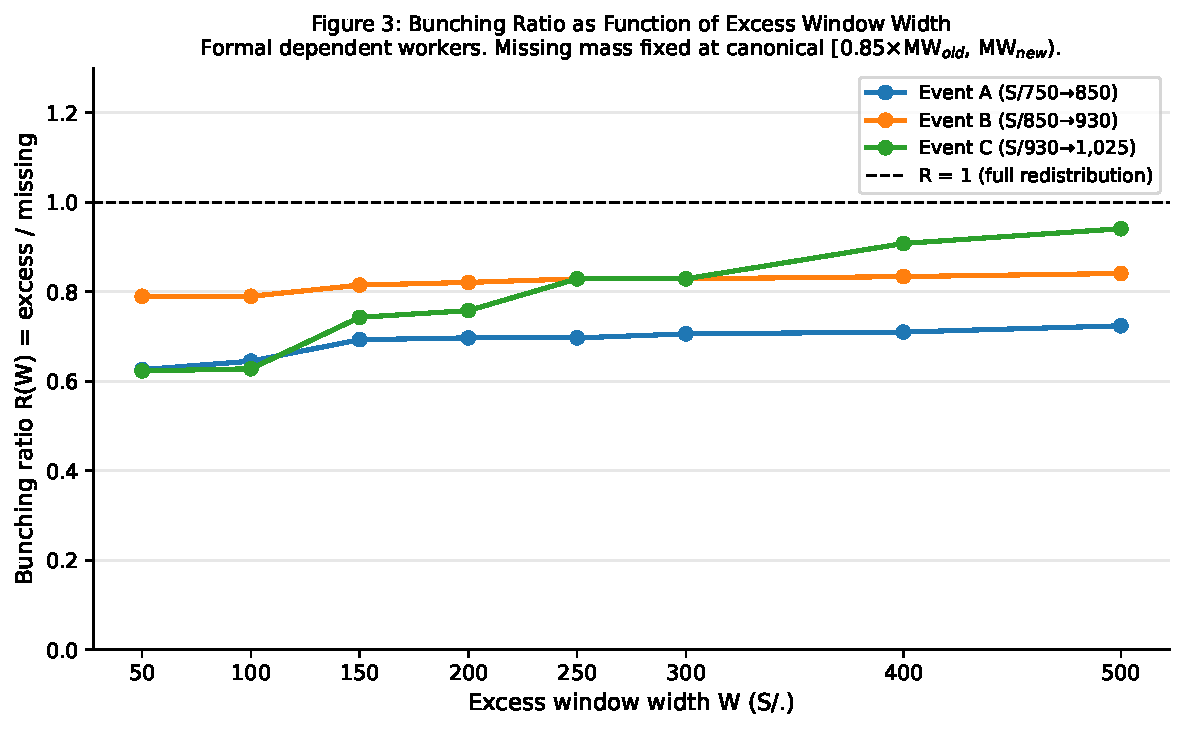
\includegraphics[width=0.85\textwidth]{../exports/figures/fig3_cumulative_excess.pdf}
\caption{Bunching Ratio $R(W)$ as a Function of Excess Window Width}
\label{fig:cumulative}
{\small \textit{Note}: Formal dependent workers (ENAHO CS). Missing mass fixed at canonical $[0.85 \times \text{MW}_\text{old}, \text{MW}_\text{new})$. Excess window $[\text{MW}_\text{new}, \text{MW}_\text{new} + W)$ varies. Dashed line at $R = 1$. Event C: pre=2021, post=2023. Background correction: inverse-absolute weighted, clean zone $> 2 \times \text{MW}_\text{new}$.}
\end{figure}

Table~\ref{tab:sensitivity} presents counterfactual sensitivity for Event B under six specifications. The canonical result ($R = 0.829$) is identical under alternative clean zone thresholds ($1.5\times$ and $2.5\times$) and under no background correction---indicating the background constant is near zero for Event B (the clean zone delta averages to essentially zero). Uniform weighting yields $R = 0.773$ ($\Delta = -0.056$); a degree-4 polynomial correction yields $R = 1.054$, as the polynomial overshoots the counterfactual in the missing zone. The range across specs is 0.773--1.054, with four of six within $\pm 0.05$ of canonical.

The polynomial result warrants explanation. A degree-4 polynomial is fitted to the post-period wage distribution in the clean zone ($> 2 \times \text{MW}_\text{new}$) and extrapolated into the affected zone as the counterfactual level. Because the polynomial must pass through the peak of the distribution---which typically occurs above 1.5$\times$MW---it extrapolates a high counterfactual into the missing zone, making the observed post-distribution appear to lie \textit{above} the counterfactual there. This generates artificially small missing mass (the zone that ``should'' have workers according to the polynomial actually does) and consequently inflates $R$ above 1. This is a well-known limitation of polynomial counterfactuals in bunching settings with sharp mass points \citep{kleven2013}: the polynomial cannot distinguish between the smooth background trend and the mass concentration created by the MW itself. The inverse-absolute weighting avoids this problem by assigning near-zero weight to bins near the MW spike and high weight to the flat upper tail, producing a counterfactual that reflects only smooth background drift.

\begin{table}[H]
\centering
\caption{Counterfactual Sensitivity --- Event B Bunching Ratio}
\label{tab:sensitivity}
\begin{threeparttable}
\small
\begin{tabular}{llccc}
\toprule
Specification & Clean zone / Weighting & Missing (pp) & Excess (pp) & $R$ \\
\midrule
Canonical          & $> 2\times\text{MW}$, inv-abs    & 7.99 & 6.62 & 0.829 \\
Uniform weights    & $> 2\times\text{MW}$, uniform    & 8.26 & 6.39 & 0.773 \\
Polynomial deg.\ 4 & $> 2\times\text{MW}$, poly fit   & 7.04 & 7.42 & 1.054 \\
Clean at $1.5\times\text{MW}$ & $> 1.5\times\text{MW}$, inv-abs & 7.99 & 6.62 & 0.829 \\
Clean at $2.5\times\text{MW}$ & $> 2.5\times\text{MW}$, inv-abs & 7.99 & 6.62 & 0.829 \\
No correction      & none                             & 7.99 & 6.62 & 0.829 \\
\bottomrule
\end{tabular}
\begin{tablenotes}
\small
\item \textit{Note}: Formal dependent workers, Event B ($\text{MW}$: S/850$\to$S/930). Missing mass from $[0.85 \times 850, 930) = [\text{S/}723, \text{S/}930)$ (negative-only bins). Excess from $[\text{S/}930, \text{S/}1{,}180)$ ($W = 250$). Background correction varies by specification. The canonical (inv-abs) and no-correction specifications give identical $R$ because the clean-zone background for Event B is near zero.
\end{tablenotes}
\end{threeparttable}
\end{table}

\begin{table}[H]
\centering
\caption{Bin Width Sensitivity --- Bunching Ratios (Formal Dependent Workers)}
\label{tab:binwidth}
\begin{threeparttable}
\small
\begin{tabular}{lcccc}
\toprule
Bin width & Boundary aligned? & $R$ (Event A) & $R$ (Event B) & $R$ (Event C) \\
          & A / B / C         &               &               &               \\
\midrule
S/10  & Y / Y / N & 0.751 & 0.836 & 0.850 \\
S/15  & N / Y / N & 0.079$^{\dagger}$ & 0.838 & 0.848 \\
S/20  & N / N / N & 0.712 & 0.804 & 0.854 \\
S/25 (canonical) & Y / N / Y & 0.697 & 0.829 & 0.829 \\
S/50  & Y / N / N & 0.677 & 0.206$^{\dagger}$ & 0.662 \\
S/100 & N / N / N & 0.477 & 0.754 & 0.613 \\
\bottomrule
\end{tabular}
\begin{tablenotes}
\small
\item \textit{Note}: Canonical inv-abs background correction; excess window S/250; formal dependent workers. ``Boundary aligned'' = $\text{MW}_\text{new} \bmod \text{BinWidth} = 0$, so the MW threshold falls on a bin edge.
\item[$\dagger$] Boundary misalignment: the bunching spike at $\text{MW}_\text{new}$ falls in a bin whose center lies below $\text{MW}_\text{new}$, classifying it as missing rather than excess. See text.
\end{tablenotes}
\end{threeparttable}
\end{table}

When the MW threshold falls on a bin boundary (aligned configurations), $R$ is stable: Event B yields 0.836 (S/10), 0.838 (S/15), and 0.829 (S/25), a range of only 0.009. Similarly, Event C gives 0.848--0.854 across aligned specifications. Misaligned configurations produce severely distorted estimates: Event A at S/15 gives $R = 0.079$ and Event B at S/50 gives $R = 0.206$, not because workers are not reappearing, but because the bunching spike at $\text{MW}_\text{new}$ lands in a bin whose center falls below the threshold, misclassifying excess as missing. At S/50, for example, $\text{MW}_\text{new} = 930$ falls in bin [900, 950) with center 925 $< 930$; workers pushed to S/930--S/949 are counted in the \textit{missing} zone rather than the excess zone. The S/25 canonical grid is the finest resolution at which both Event A (MW\textsubscript{new} = 850) and Event C (MW\textsubscript{new} = 1,025) are aligned; Event B (MW\textsubscript{new} = 930, not divisible by 25) is marginally misaligned by S/5, which does not detectably distort $R$. The narrative is therefore: $R$ stabilises at fine aligned grids (0.70--0.85) and collapses only when boundary misalignment is severe.

\textbf{Event C and COVID.} Event C's pre-period (2021) reflects post-pandemic conditions: aggregate formal employment fell 9\% in 2020 and recovered partially by 2021, with some compression of wages near the MW floor. As a robustness check, using 2019 as the pre-period (a 4-year gap) produces $R = 0.997$, compared to $R = 0.830$ with the canonical 2021 pre-period. The pre-2019 estimate reflects upward bias from economy-wide wage growth over 2019--2023 (post-pandemic recovery, headline inflation of 33\% cumulative), which shifts the entire distribution rightward and inflates measured excess mass. The canonical pre=2021 estimate is temporally proximate (8 months before the May 2022 increase) and minimizes macro confounds; the higher pre-2019 $R$ should be interpreted as an upper bound. Both estimates are consistent with the conclusion that employment effects cannot be signed.

\subsection{Wage Compression}

Table~\ref{tab:compression} presents the wage compression DiD with a decomposition into mechanical (composition) and genuine components.

\begin{table}[H]
\centering
\caption{Wage Compression DiD with Composition Decomposition}
\label{tab:compression}
\begin{threeparttable}
\begin{tabular}{lrrrrr}
\toprule
Event & Total DiD & Mechanical & Genuine & \% Mech. & New arrivals \\
\midrule
A (750$\to$850)   & $-0.035$ & $-0.028$ & $-0.008$ & 78\% & 13\% of zone \\
B (850$\to$930)   & $-0.050$ & $-0.021$ & $-0.029$ & 41\% & 10\% of zone \\
C (930$\to$1,025) & $-0.069$ & $-0.064$ & $-0.005$ & 92\% & 26\% of zone \\
\bottomrule
\end{tabular}
\begin{tablenotes}
\small
\item \textit{Note}: Compression zone = $[\text{MW}_\text{new}, 1.5 \times \text{MW}_\text{new}]$; high-wage zone = $[2 \times \text{MW}_\text{new}, 3 \times \text{MW}_\text{new}]$. Mechanical = predicted DiD from new arrivals entering at $\log(\text{MW}_\text{new})$ while existing workers grow at the high-wage rate. Genuine = total minus mechanical. With individual controls (age, sex, education, sector), the compression coefficient is $-0.045$ ($p < 0.001$).
\end{tablenotes}
\end{threeparttable}
\end{table}

For Event B, approximately 41\% of the $-0.050$ DiD reflects the composition effect---workers pushed from below the MW to the new floor entering the compression zone and diluting its mean log wage. The remaining 59\% ($-0.029$ log points) represents genuine relative wage compression. For Events A and C, the composition effect dominates (78\% and 92\%). The compression DiD is a descriptive statistic of distributional change, not a causal estimate.

\textbf{Compression robustness.} The canonical mechanical decomposition assumes new arrivals enter at exactly $\log(\text{MW}_\text{new})$ and existing compression-zone workers grow at the same rate as the high-wage control group. Table~\ref{tab:comp_robust} relaxes both assumptions for Event B. Moving the assumed entry point from $\log(930)$ to $\log(980)$ or $\log(1{,}030)$ \textit{reduces} the mechanical share (from 41\% to 31\% and 21\%), increasing the genuine compression. This is because higher entry wages are less dilutive: new arrivals pull the mean down less, so more of the observed compression must reflect genuine suppression. Similarly, if existing workers grew at only 50\% of the high-wage rate, the mechanical share rises marginally to 46\%. In all four cases, genuine compression remains negative and economically meaningful ($-0.027$ to $-0.040$ log points), confirming that the compression result is not an artifact of the canonical entry-point assumption.

\begin{table}[H]
\centering
\caption{Compression Robustness --- Mechanical vs.\ Genuine (Event B)}
\label{tab:comp_robust}
\begin{threeparttable}
\small
\begin{tabular}{lccr}
\toprule
Assumption & Mechanical & Genuine & \% Mech. \\
\midrule
1. Canonical: new arrivals at $\log(930)$     & $-0.021$ & $-0.030$ & 41\% \\
2. New arrivals at $\log(980)$                & $-0.015$ & $-0.035$ & 31\% \\
3. New arrivals at $\log(1{,}030)$            & $-0.010$ & $-0.040$ & 21\% \\
4. Existing workers grow at $50\%$ of control rate & $-0.023$ & $-0.027$ & 46\% \\
\bottomrule
\end{tabular}
\begin{tablenotes}
\small
\item \textit{Note}: Event B (S/850$\to$S/930, pre=2017, post=2019). Formal dependent workers. Total DiD fixed at $-0.050$ (observed). New arrivals = 10\% of compression zone post-period ($n_\text{new}/n_\text{post} = 0.10$). Mechanical = predicted DiD contribution from composition change; genuine = total $-$ mechanical. The high-wage growth rate $H = +0.005$ log points (from data). Entry points in assumptions 2--3 represent workers entering above the exact MW floor.
\end{tablenotes}
\end{threeparttable}
\end{table}

%=============================================================
\section{Heterogeneity}\label{sec:heterogeneity}
%=============================================================

Table~\ref{tab:hetero_industry} through Table~\ref{tab:hetero_geo} present bunching ratios across subgroups. In all panels, the Total row (0.696 / 0.829 / 0.830) matches Table~\ref{tab:bunching} exactly.

\begin{table}[H]
\centering
\caption{Bunching Ratios by Industry Sector}
\label{tab:hetero_industry}
\begin{threeparttable}
\small
\begin{tabular}{lcccc}
\toprule
Sector & Event A & Event B & Event C & Average \\
\midrule
\textbf{Total} ($N = 9{,}952$) & \textbf{0.696} & \textbf{0.829} & \textbf{0.830} & \textbf{0.785} \\
Agriculture/Mining/Utilities ($N = 1{,}031$) & 1.641 & 0.765 & 0.407 & 0.938 \\
Manufacturing ($N = 904$) & 1.000 & 0.869 & 1.049 & 0.973 \\
Commerce ($N = 937$) & 0.784 & 1.209 & 0.723 & 0.905 \\
Transport/hospitality ($N = 556$) & 1.041 & 1.018 & 0.585 & 0.881 \\
Finance/professional services ($N = 1{,}113$) & 0.768 & 1.018 & 0.806 & 0.864 \\
Public administration ($N = 1{,}639$) & 1.033 & 0.498 & 0.804 & 0.778 \\
Education and health ($N = 3{,}021$) & 0.598 & 0.709 & 0.975 & 0.760 \\
\bottomrule
\end{tabular}
\begin{tablenotes}
\small
\item \textit{Note}: $N$ = 2015 pre-period sample. Construction excluded (sparse cells, $< 500$ obs). Agriculture/Mining includes CIIU rev4 codes 35--39 (utilities). Sector from \texttt{p506r4} (CIIU 2-digit).
\end{tablenotes}
\end{threeparttable}
\end{table}

\begin{table}[H]
\centering
\caption{Bunching Ratios by Firm Size, Age, and Sex}
\label{tab:hetero_firm}
\begin{threeparttable}
\small
\begin{tabular}{lcccc}
\toprule
Group & Event A & Event B & Event C & Average \\
\midrule
\multicolumn{5}{l}{\textit{Panel B: Firm size}} \\
Micro ($\leq 10$, $N = 705$) & 0.899 & 0.909 & 0.690 & 0.833 \\
Small (11--50, $N = 1{,}238$) & 0.919 & 0.901 & 0.598 & 0.806 \\
Medium/Large (51+, $N = 7{,}557$) & 0.686 & 0.793 & 0.896 & 0.792 \\[6pt]
\multicolumn{5}{l}{\textit{Panel C: Age and sex}} \\
Age 18--24 & 0.661 & 1.010 & 0.805 & 0.826 \\
Age 25--44 & 0.748 & 0.792 & 0.797 & 0.779 \\
Age 45--64 & 0.701 & 0.927 & 0.853 & 0.827 \\
Men & 0.726 & 0.788 & 0.778 & 0.764 \\
Women & 0.697 & 0.922 & 0.877 & 0.832 \\
\bottomrule
\end{tabular}
\begin{tablenotes}
\small
\item \textit{Note}: Firm size from \texttt{p512b} (establishment worker count). Workers with missing \texttt{p512b} (4.3--5.8\% per year) are excluded from Panel B; the three rows sum to 95.5\% of the sample.
\end{tablenotes}
\end{threeparttable}
\end{table}

\begin{table}[H]
\centering
\caption{Bunching Ratios by Geography and Employer Sector}
\label{tab:hetero_geo}
\begin{threeparttable}
\small
\begin{tabular}{lcccc}
\toprule
Group & Event A & Event B & Event C & Average \\
\midrule
Lima Metropolitan ($N = 2{,}594$) & 0.618 & 1.050 & 0.817 & 0.828 \\
Rest of country ($N = 7{,}358$) & 0.856 & 0.621 & 0.888 & 0.788 \\
Urban ($N = 9{,}286$) & 0.702 & 0.843 & 0.828 & 0.791 \\
Rural ($N = 666$) & 1.016 & 0.550 & 0.909 & 0.825 \\[4pt]
Public sector ($N = 4{,}315$) & 0.921 & 0.456 & 0.865 & 0.747 \\
Private sector ($N = 5{,}576$) & 0.766 & 0.962 & 0.768 & 0.832 \\
\bottomrule
\end{tabular}
\begin{tablenotes}
\small
\item \textit{Note}: Public sector identified by \texttt{p510} $\in \{1, 2, 3\}$ or CIIU $\in \{84, 85, 86\}$.
\end{tablenotes}
\end{threeparttable}
\end{table}

Ratios cluster near 0.80 across most subgroups. The private sector absorbs MW increases more effectively (average ratio 0.832) than the public sector (0.747), where rigid pay scales limit adjustment. Manufacturing consistently shows the highest ratios ($\approx 0.97$), likely reflecting higher enforcement density. Micro firms ($\leq 10$ workers) show higher ratios than medium/large firms ($51+$ workers) in Events A and B (0.90--0.91 vs.\ 0.69--0.79), the opposite of what an enforcement story would predict. This may reflect self-selection: micro firms that are formal have already opted into compliance, while the marginal micro firm that evades formal employment entirely is excluded from the sample. No subgroup shows dramatically different behavior.

\paragraph{Interpretation caveat.} The heterogeneity analysis is descriptive, not structural. There is no exogenous variation in enforcement intensity or sector-specific MW exposure to identify why ratios differ across subgroups. The firm-size pattern (micro $>$ large in Events A--B) is inconsistent with a pure enforcement story and may reflect self-selection: micro firms that choose to formalize have already internalized compliance costs, so the marginal micro formal firm is already a high-compliance unit. The public/private gap (0.75 vs.\ 0.83) likely reflects institutional rigidity in government pay scales rather than differential MW responsiveness. These interpretations are suggestive, not causal.

\paragraph{Ethnicity.} Among formal dependent workers, indigenous (Quechua/Aymara/native-language) and non-indigenous workers have similar wage distributions (both median S/1,400) and similar MW exposure (8.5\% vs.\ 10.7\% below MW). The ethnic divide operates through access to formal employment: the indigenous formality rate is 5.7\% versus 20.7\% for Spanish speakers (a 3.6$\times$ gap). The 925 indigenous formal dependent workers are predominantly public-sector employees (59\%), concentrated in highland departments. Bunching ratios by ethnicity are unstable across events and reflect sector composition rather than differential MW compliance.

%=============================================================
\section{Hours}\label{sec:hours}
%=============================================================

Table~\ref{tab:hours} presents the intensive-margin hours DiD.

\begin{table}[H]
\centering
\caption{Weekly Hours DiD}
\label{tab:hours}
\begin{threeparttable}
\small
\begin{tabular}{lccccccr}
\toprule
Event & Treat pre & Treat post & $\Delta$ treat & Ctrl pre & Ctrl post & $\Delta$ ctrl & DiD \\
\midrule
A (750$\to$850) & 44.4h & 44.8h & +0.4h & 42.1h & 41.5h & $-$0.7h & +1.1h \\
B (850$\to$930) & 44.8h & 45.1h & +0.3h & 41.2h & 42.0h & +0.8h & $-$0.5h \\
C (930$\to$1,025) & 44.5h & 46.4h & +1.9h & 42.1h & 43.6h & +1.5h & +0.4h \\
\bottomrule
\end{tabular}
\begin{tablenotes}
\small
\item \textit{Note}: Treatment pre = workers in $[0.85 \times \text{MW}_\text{old}, \text{MW}_\text{new})$; treatment post = workers in $[\text{MW}_\text{new}, 1.3 \times \text{MW}_\text{new}]$ (bunched-up zone). Control = $[1.5 \times \text{MW}_\text{new}, 3.0 \times \text{MW}_\text{new}]$. Weighted means using \texttt{fac500a}. Variable: \texttt{p513t} (total weekly hours).
\end{tablenotes}
\end{threeparttable}
\end{table}

No DiD exceeds $\pm 1.1$h/week. There is no evidence of intensive-margin hours adjustment in response to MW increases.

%=============================================================
\section{Conclusion}\label{sec:conclusion}
%=============================================================

Peru's minimum wage increases between 2016 and 2022 produced clear, placebo-verified redistribution of the formal wage distribution. Across three events, 70--83\% of workers displaced below the old floor reappear above the new one, rising to 94\% when the excess window is extended to S/500 (Figure~\ref{fig:cumulative}). The bunching signal is specific to the true MW threshold---7$\times$ larger than at placebo thresholds (Table~\ref{tab:bunching})---stable across counterfactual specifications (Table~\ref{tab:sensitivity}), and confirmed on an independent quarterly dataset (EPE Lima, Appendix~\ref{app:epe}). Hours show no intensive-margin adjustment ($\leq \pm 1.1$h/week). Wage compression of 3--7 percentage points is present, but 41--92\% is mechanical composition; the residual genuine compression ($-0.005$ to $-0.029$ log points) is robust to alternative assumptions about where new arrivals enter (Table~\ref{tab:comp_robust}).

\textbf{Employment effects remain an open question.} The event study fails pre-trends for Events B ($p = 0.007$) and C ($p = 0.017$); Event A has no testable pre-period. The IV approach fails due to weak first stages ($F < 3$ in all events). The bunching ratios (0.70--0.83, bootstrap CIs [0.57--1.02]) are consistent with both modest displacement (up to 28\% of affected workers) and full redistribution. The data cannot distinguish between these scenarios.

Three points of external validity strengthen these findings. First, EPE Lima quarterly data produces ratios (0.73--1.03) consistent with the ENAHO results despite different formality definitions, event windows, and geographic scope. Second, placebo tests at artificial thresholds produce ratios 7 times smaller. Third, informal workers show partial response in Event A (1.218) but not in Events B--C, suggesting some spillover at lower MW levels.

This paper's central contribution is a complete diagnostic of identification in a national-MW setting: the pre-post distributional estimator recovers a clear, placebo-verified signal where three regression-based strategies---event study, Kaitz IV, and panel DiD---systematically fail. By documenting both what the data \textit{can} and \textit{cannot} identify, the paper provides a replicable template for MW analysis in developing economies without sub-national MW variation. This is not a data-quality failure---it is a structural feature of single-national-MW settings. The cross-sectional design cannot decompose the missing mass into transitions to informality versus exit from employment---a distinction with important policy implications. Future work using administrative wage registries (SUNAT, ESSALUD) would allow this decomposition through quarterly firm-level job flows, substantially improving both the power to detect employment effects and the ability to trace where displaced workers go.

%=============================================================
% REFERENCES
%=============================================================
\newpage
\bibliographystyle{aer}
\bibliography{mw_paper}

%=============================================================
% APPENDICES
%=============================================================
\newpage
\begin{appendices}

\section{ENAHO Panel 978 --- Event C}\label{app:panel}

The ENAHO panel 978 tracks a subsample of individuals from 2021 to 2023. Treatment: formal dependent workers in 2021 with wages in [S/791, S/1,025). Control: wages in [S/1,230, S/2,563]. Approximately 76\% of both groups are not re-interviewed; results apply to the surviving 24\% only. Outcome statistics are weighted by \texttt{facpanel2123}. Attrited workers are \textit{not} counted as non-employed.

\begin{table}[H]
\centering
\caption{Panel Transition Results (Event C, 2021$\to$2023)}
\label{tab:panel}
\begin{threeparttable}
\small
\begin{tabular}{lccc}
\toprule
Metric & Treatment ($N = 1{,}171$) & Control ($N = 3{,}903$) & DiD \\
\midrule
Re-interviewed rate & 24.4\% & 23.6\% & --- \\
\multicolumn{4}{l}{\textit{Among re-interviewed (weighted):}} \\
\quad Employment retention & 63.9\% & 60.1\% & +3.8pp \\
\quad Formal dep retention & 46.8\% & 49.9\% & $-$3.1pp \\
\quad $\Delta$ log wage (stayers) & +0.307 & +0.154 & +0.153 \\
\quad $\Delta$ hours (stayers) & +0.7h & $-$1.3h & +2.0h \\
\bottomrule
\end{tabular}
\begin{tablenotes}
\small
\item \textit{Caveat}: 76\% attrition with differential selection ($p = 0.022$). Do not interpret causally.
\end{tablenotes}
\end{threeparttable}
\end{table}

\section{Event Study --- Pre-Trend Violations}\label{app:eventstudy}

All three events have identification problems. Event A: no prior years available (2015 = base); parallel trends untestable. Event B: joint pre-trend $F$-test $p = 0.007$; higher-Kaitz departments had systematically higher employment before the MW change. Event C: joint pre-trend $p = 0.017$; pre-COVID Kaitz--employment correlation renders the comparison non-parallel.

\section{IV / OWE --- Not Identified}\label{app:iv}

Three IV approaches were tested. (1) Department-level Kaitz IV: $F = 1.5 / 2.6 / 0.1$ across events, all far below the Stock-Yogo threshold. (2) Province-level IV: $F = 11.72$ for Event B but with reversed first-stage sign and failed pre-trends. (3) Within-year province IV: $F = 16.15$ but the placebo (no-MW-change year) produces $F = 12.71$---the instrument captures seasonal wage dynamics, not MW exposure.

\begin{table}[H]
\centering
\caption{Department-Level Kaitz IV}
\label{tab:iv}
\begin{threeparttable}
\small
\begin{tabular}{lrrrrrrr}
\toprule
Event & $\hat{\pi}$ (FS) & SE & $F$ & $\hat{\beta}$ (RF) & SE & OWE & SE \\
\midrule
A & +0.169 & 0.082 & 1.5 & +0.014 & 0.038 & +0.082 & 0.229 \\
B & $-$0.070 & 0.103 & 2.6 & +0.122 & 0.044 & --- & --- \\
C & +0.132 & 0.090 & 0.1 & +0.220 & 0.076 & +1.667 & 1.271 \\
\bottomrule
\end{tabular}
\begin{tablenotes}
\small
\item \textit{Note}: Event B OWE not reported (reversed first-stage sign). SE clustered by department (24 clusters). All $F < 3$; instrument is weak.
\end{tablenotes}
\end{threeparttable}
\end{table}

\section{EPEN CIU Annual 2023 --- Lee-Saez Bunching}\label{app:epen}

Single-period Lee-Saez estimate from INEI code 873 ($N = 53{,}316$ formal urban workers). All cities show excess mass at MW: ratio 1.622. These are not directly comparable to the pre-post ratios in Table~\ref{tab:bunching}.

\section{EPE Lima Quarterly Bunching}\label{app:epe}

EPE Lima provides an independent dataset check with tighter 6-month event windows (Q1 vs.\ Q3 of each event year). Formality uses \texttt{p222 == 1} (EsSalud only), which is narrower than ENAHO. Lima Metropolitan Area only.

\begin{table}[H]
\centering
\caption{EPE Lima Pre-Post Bunching (6-Month Windows)}
\label{tab:epe}
\begin{threeparttable}
\small
\begin{tabular}{llrrrcccc}
\toprule
Event & Window & $N$ pre & $N$ post & Near-MW & Ratio & 95\% CI & ENAHO \\
\midrule
A & Q1$\to$Q3 2016 & 2,622 & 2,599 & 240 & 1.031 & [0.70, 1.63] & 0.696 \\
B & Q1$\to$Q3 2018 & 2,280 & 2,438 & 302 & 0.733 & [0.60, 1.03] & 0.829 \\
C & Q1$\to$Q3 2022 & 1,933 & 1,936 & 331 & 0.885 & [0.70, 1.13] & 0.830 \\
\bottomrule
\end{tabular}
\begin{tablenotes}
\small
\item \textit{Note}: All ENAHO ratios fall within EPE Lima bootstrap CIs. Event A diverges in point estimates; Lima's lower Kaitz may explain the higher absorption rate. CIs wide due to small $N$.
\end{tablenotes}
\end{threeparttable}
\end{table}

\end{appendices}

\end{document}
